% Options for packages loaded elsewhere
\PassOptionsToPackage{unicode}{hyperref}
\PassOptionsToPackage{hyphens}{url}
%
\documentclass[
  english,
  man,floatsintext]{apa6}
\usepackage{lmodern}
\usepackage{amssymb,amsmath}
\usepackage{ifxetex,ifluatex}
\ifnum 0\ifxetex 1\fi\ifluatex 1\fi=0 % if pdftex
  \usepackage[T1]{fontenc}
  \usepackage[utf8]{inputenc}
  \usepackage{textcomp} % provide euro and other symbols
\else % if luatex or xetex
  \usepackage{unicode-math}
  \defaultfontfeatures{Scale=MatchLowercase}
  \defaultfontfeatures[\rmfamily]{Ligatures=TeX,Scale=1}
\fi
% Use upquote if available, for straight quotes in verbatim environments
\IfFileExists{upquote.sty}{\usepackage{upquote}}{}
\IfFileExists{microtype.sty}{% use microtype if available
  \usepackage[]{microtype}
  \UseMicrotypeSet[protrusion]{basicmath} % disable protrusion for tt fonts
}{}
\makeatletter
\@ifundefined{KOMAClassName}{% if non-KOMA class
  \IfFileExists{parskip.sty}{%
    \usepackage{parskip}
  }{% else
    \setlength{\parindent}{0pt}
    \setlength{\parskip}{6pt plus 2pt minus 1pt}}
}{% if KOMA class
  \KOMAoptions{parskip=half}}
\makeatother
\usepackage{xcolor}
\IfFileExists{xurl.sty}{\usepackage{xurl}}{} % add URL line breaks if available
\IfFileExists{bookmark.sty}{\usepackage{bookmark}}{\usepackage{hyperref}}
\hypersetup{
  pdftitle={Peekbank: Exploring children's word recognition through an open, large-scale repository for developmental eye-tracking data},
  pdfauthor={Peekbank team2, Martin Zettersten1, Claire Bergey2, Naiti S. Bhatt3, Veronica Boyce4, Mika Braginsky5, Alexandra Carstensen4, Benny deMayo1, George Kachergis4, Molly Lewis6, Bria Long4, Kyle MacDonald7, Jessica Mankewitz4, Stephan Meylan5,8, Annissa N. Saleh9, Rose M. Schneider10, Angeline Sin Mei Tsui4, Sarp Uner8, Tian Linger Xu11, Daniel Yurovsky6, \& Michael C. Frank1},
  pdflang={en-EN},
  pdfkeywords={keywords},
  hidelinks,
  pdfcreator={LaTeX via pandoc}}
\urlstyle{same} % disable monospaced font for URLs
\usepackage{graphicx,grffile}
\makeatletter
\def\maxwidth{\ifdim\Gin@nat@width>\linewidth\linewidth\else\Gin@nat@width\fi}
\def\maxheight{\ifdim\Gin@nat@height>\textheight\textheight\else\Gin@nat@height\fi}
\makeatother
% Scale images if necessary, so that they will not overflow the page
% margins by default, and it is still possible to overwrite the defaults
% using explicit options in \includegraphics[width, height, ...]{}
\setkeys{Gin}{width=\maxwidth,height=\maxheight,keepaspectratio}
% Set default figure placement to htbp
\makeatletter
\def\fps@figure{htbp}
\makeatother
\setlength{\emergencystretch}{3em} % prevent overfull lines
\providecommand{\tightlist}{%
  \setlength{\itemsep}{0pt}\setlength{\parskip}{0pt}}
\setcounter{secnumdepth}{-\maxdimen} % remove section numbering
% Make \paragraph and \subparagraph free-standing
\ifx\paragraph\undefined\else
  \let\oldparagraph\paragraph
  \renewcommand{\paragraph}[1]{\oldparagraph{#1}\mbox{}}
\fi
\ifx\subparagraph\undefined\else
  \let\oldsubparagraph\subparagraph
  \renewcommand{\subparagraph}[1]{\oldsubparagraph{#1}\mbox{}}
\fi
% Manuscript styling
\usepackage{upgreek}
\captionsetup{font=singlespacing,justification=justified}

% Table formatting
\usepackage{longtable}
\usepackage{lscape}
% \usepackage[counterclockwise]{rotating}   % Landscape page setup for large tables
\usepackage{multirow}		% Table styling
\usepackage{tabularx}		% Control Column width
\usepackage[flushleft]{threeparttable}	% Allows for three part tables with a specified notes section
\usepackage{threeparttablex}            % Lets threeparttable work with longtable

% Create new environments so endfloat can handle them
% \newenvironment{ltable}
%   {\begin{landscape}\begin{center}\begin{threeparttable}}
%   {\end{threeparttable}\end{center}\end{landscape}}
\newenvironment{lltable}{\begin{landscape}\begin{center}\begin{ThreePartTable}}{\end{ThreePartTable}\end{center}\end{landscape}}

% Enables adjusting longtable caption width to table width
% Solution found at http://golatex.de/longtable-mit-caption-so-breit-wie-die-tabelle-t15767.html
\makeatletter
\newcommand\LastLTentrywidth{1em}
\newlength\longtablewidth
\setlength{\longtablewidth}{1in}
\newcommand{\getlongtablewidth}{\begingroup \ifcsname LT@\roman{LT@tables}\endcsname \global\longtablewidth=0pt \renewcommand{\LT@entry}[2]{\global\advance\longtablewidth by ##2\relax\gdef\LastLTentrywidth{##2}}\@nameuse{LT@\roman{LT@tables}} \fi \endgroup}

% \setlength{\parindent}{0.5in}
% \setlength{\parskip}{0pt plus 0pt minus 0pt}

% \usepackage{etoolbox}
\makeatletter
\patchcmd{\HyOrg@maketitle}
  {\section{\normalfont\normalsize\abstractname}}
  {\section*{\normalfont\normalsize\abstractname}}
  {}{\typeout{Failed to patch abstract.}}
\patchcmd{\HyOrg@maketitle}
  {\section{\protect\normalfont{\@title}}}
  {\section*{\protect\normalfont{\@title}}}
  {}{\typeout{Failed to patch title.}}
\makeatother
\shorttitle{Peekbank repository for developmental eye-tracking data}
\keywords{keywords\newline\indent Word count: X}
\DeclareDelayedFloatFlavor{ThreePartTable}{table}
\DeclareDelayedFloatFlavor{lltable}{table}
\DeclareDelayedFloatFlavor*{longtable}{table}
\makeatletter
\renewcommand{\efloat@iwrite}[1]{\immediate\expandafter\protected@write\csname efloat@post#1\endcsname{}}
\makeatother
\usepackage{lineno}

\linenumbers
\usepackage{csquotes}
\ifxetex
  % Load polyglossia as late as possible: uses bidi with RTL langages (e.g. Hebrew, Arabic)
  \usepackage{polyglossia}
  \setmainlanguage[]{english}
\else
  \usepackage[shorthands=off,main=english]{babel}
\fi

\title{Peekbank: Exploring children's word recognition through an open, large-scale repository for developmental eye-tracking data}
\author{Peekbank team\textsuperscript{2}, Martin Zettersten\textsuperscript{1}, Claire Bergey\textsuperscript{2}, Naiti S. Bhatt\textsuperscript{3}, Veronica Boyce\textsuperscript{4}, Mika Braginsky\textsuperscript{5}, Alexandra Carstensen\textsuperscript{4}, Benny deMayo\textsuperscript{1}, George Kachergis\textsuperscript{4}, Molly Lewis\textsuperscript{6}, Bria Long\textsuperscript{4}, Kyle MacDonald\textsuperscript{7}, Jessica Mankewitz\textsuperscript{4}, Stephan Meylan\textsuperscript{5,8}, Annissa N. Saleh\textsuperscript{9}, Rose M. Schneider\textsuperscript{10}, Angeline Sin Mei Tsui\textsuperscript{4}, Sarp Uner\textsuperscript{8}, Tian Linger Xu\textsuperscript{11}, Daniel Yurovsky\textsuperscript{6}, \& Michael C. Frank\textsuperscript{1}}
\date{}


\authornote{

Add complete departmental affiliations for each author here. Each new line herein must be indented, like this line.

Enter author note here.

The authors made the following contributions. Peekbank team: Conceptualization, Writing - Original Draft Preparation, Writing - Review \& Editing.

Correspondence concerning this article should be addressed to Peekbank team, Postal address. E-mail: \href{mailto:my@email.com}{\nolinkurl{my@email.com}}

}

\affiliation{\vspace{0.5cm}\textsuperscript{1} Dept. of Psychology, Princeton University\\\textsuperscript{2} Dept. of Psychology, University of Chicago\\\textsuperscript{3} Scripps College\\\textsuperscript{4} Dept. of Psychology, Stanford University\\\textsuperscript{5} Dept. of Brain and Cognitive Sciences, MIT\\\textsuperscript{6} Dept. of Psychology, Carnegie Mellon University\\\textsuperscript{7} Core Technology, McD Tech Labs\\\textsuperscript{8} Dept. of Psychology and Neuroscience, Duke University\\\textsuperscript{9} Dept. of Psychology, UT Austin\\\textsuperscript{10} Dept. of Psychology, UC San Diego\\\textsuperscript{11} Dept. of Psychological and Brain Sciences, Indiana University}

\abstract{
The ability to rapidly recognize words and link them to referents in context is central to children's early language development.
This ability, often called word recognition in the developmental literature, is typically studied in the looking-while-listening paradigm, which measures infants' fixation on a target object (vs.~a distractor) after hearing a target label.
We present a large-scale, open database of infant and toddler eye-tracking data from looking-while-listening tasks.
The goal of this effort is to address theoretical and methodological challenges in measuring vocabulary development.
{[}tools; processing; analysis/ usage examples{]}
}



\begin{document}
\maketitle

\hypertarget{introduction}{%
\section{Introduction}\label{introduction}}

Across their first years of life, children learn words in their native tongues at a rapid pace (Frank, Braginsky, Yurovsky, \& Marchman, 2021).
{[}notes about the size/ pace{]}
A key part of the word learning process is children's emerging ability to rapidly process words and link them to relevant meanings -- often referred to as word recognition.
Measuring early word recognition offers insight into children's early word representations and the processes supporting early language comprehension (Bergelson, 2020).
Word recognition skills are also thought to build a foundation for children's subsequent language development.
Past research has found that early word recognition efficiency is predictive of later linguistic and general cognitive outcomes (Bleses, Makransky, Dale, Højen, \& Ari, 2016; Marchman et al., 2018).
While word recognition is a central part of children's language development, mapping the trajectory of word recognition skills has remained elusive.
Studies investigating children's word recognition are typically limited in scope to experiments in individual labs involving small samples tested on a limited set of items.
This limitation in scale makes it difficult to understand developmental changes in children's word knowledge at a broad scale.
Peekbank provides an openly accessible database of eye-tracking data of children's word recognition, with the primary goal of facilitating the study of developmental changes in children's word knowledge and recognition speed.

\hypertarget{the-looking-while-listening-paradigm}{%
\subsection{\texorpdfstring{The \enquote{Looking-While-Listening} Paradigm}{The ``Looking-While-Listening'' Paradigm}}\label{the-looking-while-listening-paradigm}}

Word recognition is traditionally studied in the \enquote{looking-while-listening} paradigm (alternatively referred to as the intermodal preferential looking procedure; Fernald, Zangl, Portillo, \& Marchman, 2008; Hirsh-Pasek, Cauley, Golinkoff, \& Gordon, 1987).
In such studies, infants listen to a sentence prompting a specific referent (e.g., Look at the dog!) while viewing two images on the screen (e.g., an image of a dog -- the target image -- and an image of a duck -- the distractor image).
Infants' word recognition is measured in terms of how quickly and accurately they fixate on the correct target image after hearing its label.
Past research has used this same basic method to study a wide range of questions in language development.
For example, the looking-while-listening paradigm has been used to uncover early knowledge of nouns in infants' early noun knowledge, phonological representations of words, prediction during language processing, and individual differences in language development (Bergelson \& Swingley, 2012; Golinkoff, Ma, Song, \& Hirsh-Pasek, 2013; Lew-Williams \& Fernald, 2007; Marchman et al., 2018; Swingley \& Aslin, 2000).

\hypertarget{measuring-developmental-change-in-word-recognition}{%
\subsection{Measuring developmental change in word recognition}\label{measuring-developmental-change-in-word-recognition}}

While the looking-while-listening paradigm has been highly fruitful in advancing understanding of early word knowledge, fundamental questions remain both about the trajectory of children's word recognition ability and the nature of the method itself.
One central question is how to measure developmental change in word recognition.
A key idea in the language learning literature is that processing speed - the ability to quickly link a word with its referent - supports language learning.
Age-related changes in speed of processing are thought to accelerate infants' subsequent language learning: the faster infants are able to process incoming speech input, the better able they become to learn from their language environment.
Similarly, longitudinal analyses have found that individual differences in word recognition speed predict linguistic and cognitive outcomes later in childhood (e.g., Marchman \& Fernald, 2008).
However, measuring increases in the speed and accuracy of word recognition faces the challenge of distinguishing developmental changes in word recognition skill from changes in knowledge of specific words.
This problem is particularly thorny in child development, since the number of items that can be tested within a single session is limited and items must be selected in an age-appropriate manner (Peter et al., 2019).
Measuring developmental change therefore requires large-scale datasets with a range of items, in order to generalize age-related changes across words.

\hypertarget{developing-methodological-best-practices}{%
\subsection{Developing methodological best-practices}\label{developing-methodological-best-practices}}

A second question relates to evaluating methodological best practices. In particular, many fundamental analytic decisions vary substantially across studies, and different decisions may lead to different inferences about children's word recognition. For example, researchers vary in how they select time windows for analysis, transform the dependent measure of target fixations, and model the time course of word recognition (Csibra, Hernik, Mascaro, Tatone, \& Lengyel, 2016; Fernald et al., 2008; Huang \& Snedeker, 2020). This problem is made more complex by the fact that many of these decisions depend on a variety of design-related and participant-related factors (e.g., infant age). Establishing best practices therefore requires a large database of infant word recognition studies varying across such factors, in order to test the potential consequences of methodological decisions on study results.

\hypertarget{peekbank-an-open-database-of-developmental-eye-tracking-studies.}{%
\subsection{Peekbank: An open database of developmental eye-tracking studies.}\label{peekbank-an-open-database-of-developmental-eye-tracking-studies.}}

What these two questions share is that they are difficult to answer at the scale of a single study. To address this challenge, we introduce Peekbank, a flexible and reproducible interface to an open database of developmental eye-tracking studies. The Peekbank project (a) collects a large set of eye-tracking datasets on children's word recognition, (b) introduces a data format and processing tools for standardizing eye-tracking data across data sources, and (c) provides an interface for accessing and analyzing the database. In the current paper, we give an overview of the key components of the project and some initial demonstrations of its utility in advancing theoretical and methodological insights. We report two analyses using the database and associated tools (N=1,233): (1) a growth curve analysis modeling age-related changes in infants' word recognition while generalizing across item-level variability; and (2) a multiverse-style analysis of how a central methodological decision -- selecting the time window of analysis -- impacts inter-item reliability.

\hypertarget{design-and-technical-approach}{%
\section{Design and Technical Approach}\label{design-and-technical-approach}}

\hypertarget{database-framework.}{%
\subsection{Database Framework.}\label{database-framework.}}

The Peekbank data framework consists of three components: (1) processing raw experimental datasets; (2) populating a relational database; and (3) providing an interface to the database (Fig XX). The peekds library (for the R language; R Development Core Team, 2020) helps researchers convert and validate existing datasets to use the relational format of the database. The peekbank module (Python) creates a database with the relational schema and populates it with the standardized datasets produced by peekds. The database is implemented in MySQL, an industry standard relational database, which may be accessed by a variety of programming languages over the internet. The peekbankr library (R) provides an application programming interface, or API, that offers high-level abstractions for accessing data in Peekbank.

\begin{figure}

{\centering 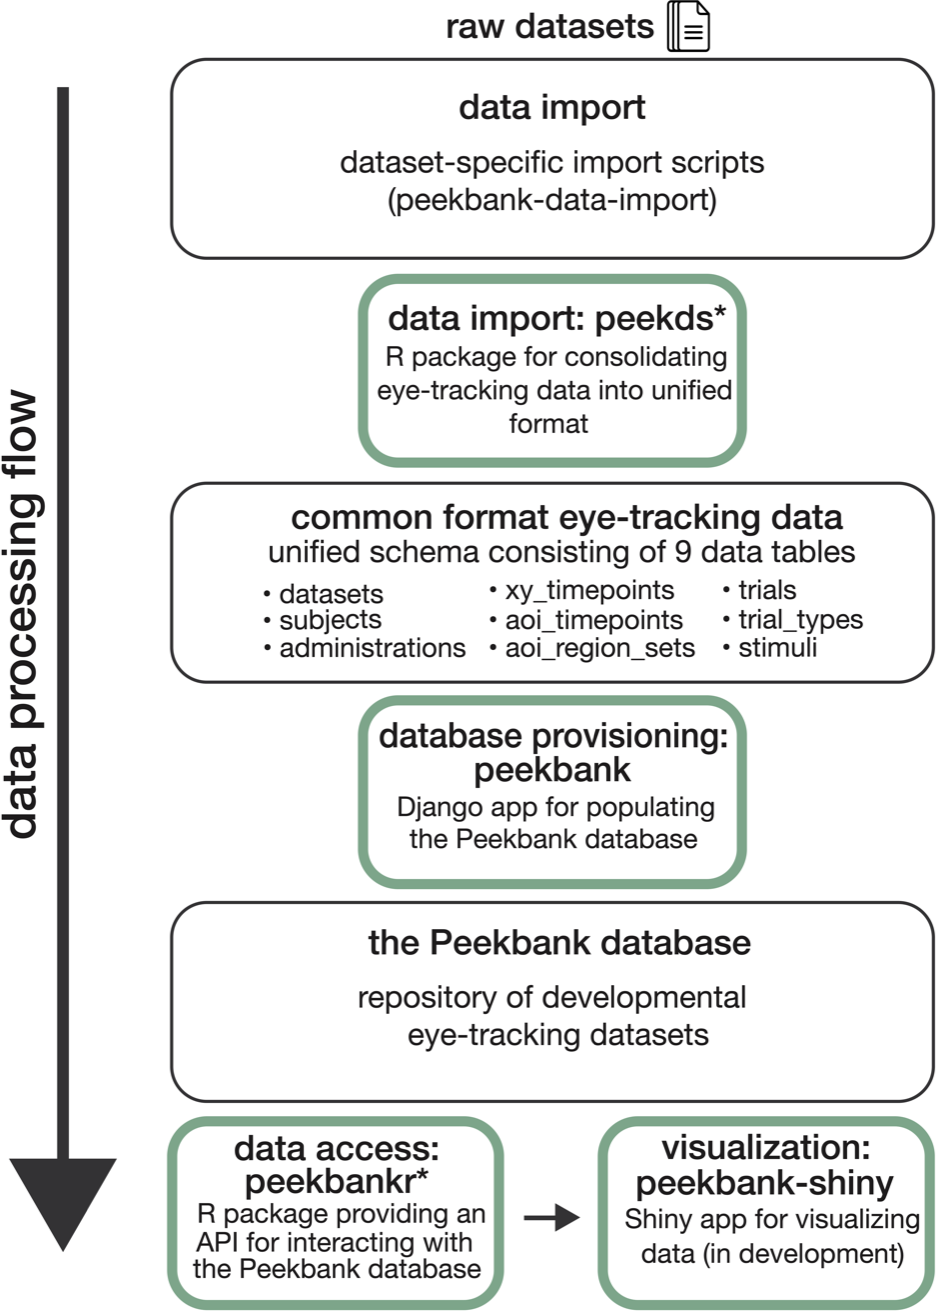
\includegraphics{peekbank-brm_files/figure-latex/fig-framework-overview-1} 

}

\caption{Overview of the Peekbank data ecosystem. Peekbank tools are highlighted in green. *custom R packages.}\label{fig:fig-framework-overview}
\end{figure}

\hypertarget{data-format-and-processing.}{%
\subsection{Data Format and Processing.}\label{data-format-and-processing.}}

One of the main challenges in compiling a large-scale eye-tracking dataset is the lack of a shared re-usable data format across individual experiments. Researcher conventions for structuring data vary, as do the technical specifications of different devices, rendering the task of integrating datasets from different labs and data sources difficult. We developed a common, tidy format for the eye-tracking data in Peekbank to ease the process of conducting cross-dataset analyses (Wickham et al., 2019). The schema of the database is sufficiently general to handle heterogeneous datasets, including both manually coded and automated eye-tracking data.

\begin{figure}

{\centering 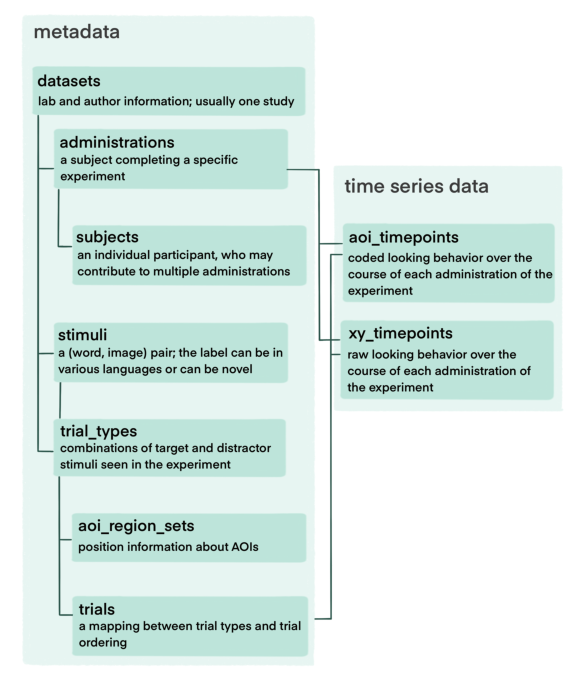
\includegraphics{peekbank-brm_files/figure-latex/fig-schema-1} 

}

\caption{The Peekbank schema. Each square represents a table in the relational database.}\label{fig:fig-schema}
\end{figure}

During data import, raw eye-tracking datasets are processed to conform to the Peekbank data schema. The centerpiece of the schema is the aoi\_timepoints table (Fig XX), which records whether participants looked to the target or the distractor stimulus at each timepoint of a given trial. Additional tables track information about data sources, participant characteristics, trial characteristics, stimuli, and raw eye-tracking data. In addition to unifying the data format, we conduct several additional pre-processing steps to facilitate analyses across datasets, including resampling observations to a common sampling rate (40 Hz) and normalizing time relative to the onset of the target label.

\hypertarget{current-data-sources.}{%
\subsection{Current Data Sources.}\label{current-data-sources.}}

\begin{table}[ht]
\centering
\begingroup\fontsize{9pt}{10pt}\selectfont
\begin{tabular}{lrrrrrr}
  \hline
Dataset Name & Citation & N & Mean Age (mos.) & Age Range (mos.) & Method & Language \\ 
  \hline
attword & (Yurovsky \& Frank, 2017) & 288 & 25.5 & 13 - 59 & eye-tracking & English \\ 
  canine & unpublished & 36 & 23.8 & 21 - 27 & manual coding & English \\ 
  coartic & (Mahr et al., 2015) & 29 & 20.8 & 18 - 24 & eye-tracking & English \\ 
  cowpig & (Perry et al., 2017) & 45 & 20.5 & 19 - 22 & manual coding & English \\ 
  ft\_pt & (Adams et al., 2018) & 69 & 17.1 & 13 - 20 & manual coding & English \\ 
  mispron & (Swingley \& Aslin, 2002) & 50 & 15.1 & 14 - 16 & manual coding & English \\ 
  mix & (Byers-Heinlein et al., 2017) & 48 & 20.1 & 19 - 21 & eye-tracking & English, French \\ 
  reflook\_socword & (Yurovsky et al., 2013) & 435 & 33.6 & 12 - 70 & eye-tracking & English \\ 
  reflook\_v4 & unpublished & 45 & 34.2 & 11 - 60 & eye-tracking & English \\ 
  remix & (Potter et al., 2019) & 44 & 22.6 & 18 - 29 & manual coding & Spanish, English \\ 
  salientme & (Pomper \& Saffran, 2019) & 44 & 40.1 & 38 - 43 & manual coding & English \\ 
  switchingCues & (Pomper \& Saffran, 2016) & 60 & 44.3 & 41 - 47 & manual coding & English \\ 
  tablet & (Frank et al., 2016) & 69 & 35.5 & 12 - 60 & eye-tracking & English \\ 
  tseltal & (Casillas et al., 2017) & 23 & 31.3 & 9 - 48 & manual coding & Tseltal \\ 
  yoursmy & (Garrison et al., 2020) & 35 & 14.5 & 12 - 18 & eye-tracking & English \\ 
   \hline
\end{tabular}
\endgroup
\caption{Overview over the datasets in the current database.} 
\end{table}

The database currently includes 11 looking-while-listening datasets comprising \emph{N}=1320 total participants (Table XX). Most datasets (10 out of 11 total) consist of data from monolingual native English speakers. They span a wide age spectrum with participants ranging from 8 to 84 months of age, and are balanced in terms of gender (48\% female). The datasets vary across a number of dimensions related to design and methodology, and include studies using manually coded video recordings and automated eye-tracking methods (e.g., Tobii, EyeLink) to measure gaze behavior. Most studies focused on testing familiar items, but the database also includes studies with novel pseudowords. All data (and accompanying references) are openly available on the Open Science Framework (\url{https://osf.io/pr6wu/?view_only=07a3887eb7a24643bdc1b2612f2729de}).

How selected?
Language coverage?
More details about lab and design variation?

\hypertarget{versioning-expanding-the-database}{%
\subsection{Versioning + Expanding the database}\label{versioning-expanding-the-database}}

Information about versioning approach/ regularity of updates
Steps for extending the database?

\hypertarget{interfacing-with-peekbank}{%
\section{Interfacing with peekbank}\label{interfacing-with-peekbank}}

\hypertarget{shiny-app}{%
\subsection{Shiny App}\label{shiny-app}}

One goal of the Peekbank project is to allow a wide range of users to easily explore and learn from the database.
We therefore have created an interactive web application -- \texttt{peekbank-shiny} -- that allows users to quickly and easily create informative visualizations of individual datasets and aggregated data.
\texttt{peekbank-shiny} is built using Shiny, a software package for creating web apps using R.
The Shiny app allows users to create commonly used visualizations of looking-while-listening data, based on data from the Peekbank database.
Specifically, users can visualize

\begin{enumerate}
\def\labelenumi{\arabic{enumi}.}
\tightlist
\item
  the time course of looking data in a profile plot depicting infant target looking across trial time,
\item
  overall accuracy (proportion target looking) within a specified analysis window,
\item
  reaction times (speed of fixating the target image) in response to a target label, and
\item
  an onset-contingent plot, which shows the time course of participant looking as a function of their look location at the onset of the target label.
\end{enumerate}

Users are given various customization options for each of these visualizations, e.g., choosing which datasets to include in the plots, controlling the age range of participants, splitting the visualizations by age bins, and controlling the analysis window for time course analyses.
Plots are then updated in real time to reflect users' customization choices, and users are given options to share the visualizations they created.
The Shiny app thus allows users to quickly inspect basic properties of Peekbanks datasets and create reproducible visualizations without incurring any of the technical overhead required to access the database through R.

\hypertarget{peekbankr}{%
\subsection{Peekbankr}\label{peekbankr}}

Functions:
connect\_to\_peekbank():
get\_datasets()
get\_subjects()
get\_administrations()
get\_stimuli()
get\_aoi\_timepoints()
get\_trials()
get\_trial\_types()
get\_xy\_timepoints()
get\_aoi\_region\_sets()

\hypertarget{osf-site}{%
\subsection{OSF site}\label{osf-site}}

Stimuli
Data in raw format (if some additional datum needed, e.g.~pupil size?)

\hypertarget{peekbank-in-action}{%
\section{Peekbank in Action}\label{peekbank-in-action}}

We provide two potential use-cases for Peekbank data. In each case, we provide sample code so as to model how easy it is to do simple analyses using data from the database. Our first example shows how we can replicate the analysis for a classic study. This type of computational reproducibility can be a very useful exercise for teaching students about best practices for data analysis (e.g., {\textbf{???}}) and also provides an easy way to explore looking-while-listening timecourse data in a standardized format. Our second example showss an in-depth exploration of developmental changes in the recognition of particular words. Besides its theoretical interest (which we will explore more fully in subsequent work), this type of analysis can be used for optimizing the stimuli for new experiments.

\hypertarget{computational-reproducibility-example-swingley-aslin-2002}{%
\subsection{Computational reproducibility example: Swingley \& Aslin (2002)}\label{computational-reproducibility-example-swingley-aslin-2002}}

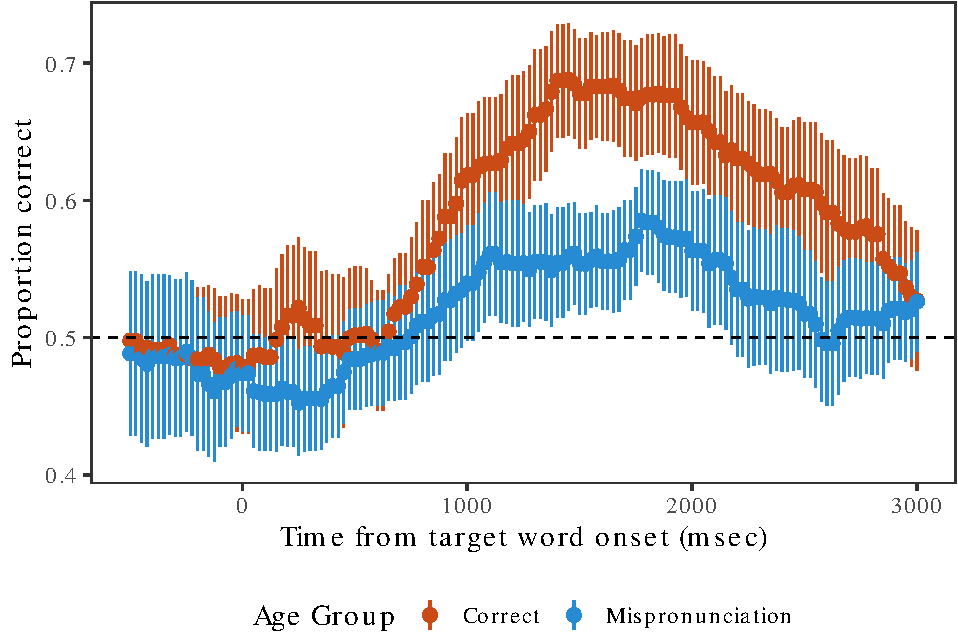
\includegraphics{peekbank-brm_files/figure-latex/unnamed-chunk-1-1.pdf}

\hypertarget{item-analyses}{%
\subsection{Item analyses}\label{item-analyses}}

To illustrate the power of aggregating data across multiple datasets, we,

aspirational goal -

ALso, item selection but maybe not yet?

\hypertarget{links-to-parent-report-vocabulary-data}{%
\subsection{Links to parent report vocabulary data}\label{links-to-parent-report-vocabulary-data}}

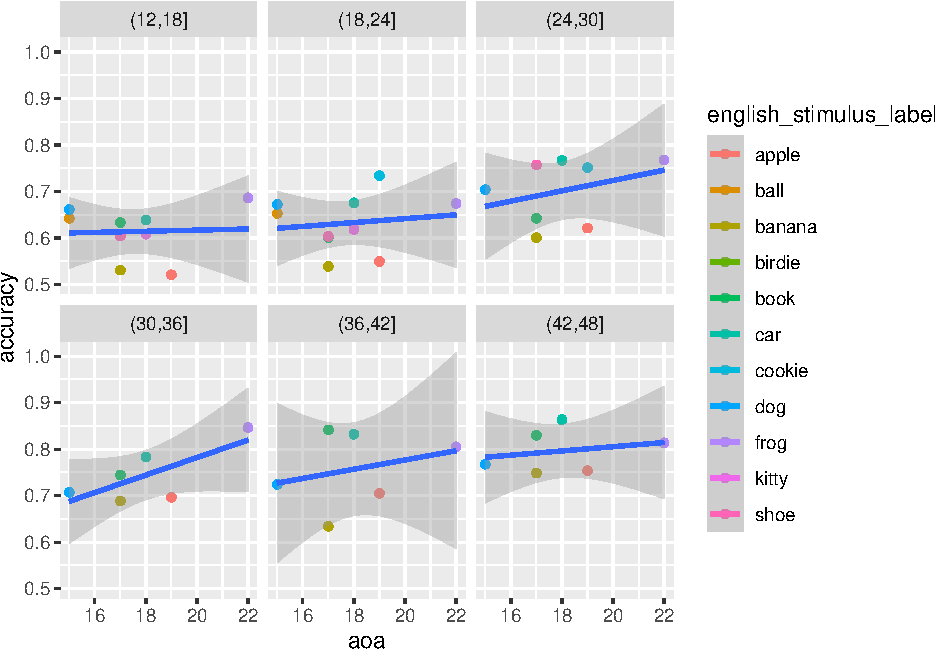
\includegraphics{peekbank-brm_files/figure-latex/unnamed-chunk-5-1.pdf}

\hypertarget{discussion-conclusion}{%
\section{Discussion/ Conclusion}\label{discussion-conclusion}}

Theoretical progress in understanding child development requires rich datasets, but collecting child data is expensive, difficult, and time-intensive. Recent years have seen a growing effort to build open source tools and pool research efforts to meet the challenge of building a cumulative developmental science (Bergmann et al., 2018; Frank, Braginsky, Yurovsky, \& Marchman, 2017; The ManyBabies Consortium, 2020). The Peekbank project expands on these efforts by building an infrastructure for aggregating eye-tracking data across studies, with a specific focus on the looking-while-listening paradigm. This paper presents an illustration of some of the key theoretical and methodological questions that can be addressed using Peekbank: generalizing across item-level variability in children's word recognition and providing data-driven guidance on methodological choices.

There are a number of limitations surrounding the current scope of the database. A priority in future work will be to expand the size of the database. With 11 datasets currently available in the database, idiosyncrasies of particular designs and condition manipulations still have substantial influence on modeling results. Expanding the set of distinct datasets will allow us to increase the number of observations per item across datasets, leading to more robust generalizations across item-level variability. The current database is also limited by the relatively homogeneous background of its participants, both with respect to language (almost entirely monolingual native English speakers) and cultural background (all but one dataset comes from WEIRD populations; Muthukrishna et al., 2020). Increasing the diversity of participant backgrounds and languages will expand the scope of the generalizations we can form about child word recognition.
Finally, while the current database is focused on studies of word recognition, the tools and infrastructure developed in the project can in principle be used to accommodate any eye-tracking paradigm, opening up new avenues for insights into cognitive development. Gaze behavior has been at the core of many of the key advances in our understanding of infant cognition. Aggregating large datasets of infant looking behavior in a single, openly-accessible format promises to bring a fuller picture of infant cognitive development into view.

\hypertarget{acknowledgements}{%
\section{Acknowledgements}\label{acknowledgements}}

We would like to thank the labs and researchers that have made their data publicly available in the database.

We used R (Version 4.0.3; R Core Team, 2020) and the R-packages \emph{dplyr} (Version 1.0.3; Wickham et al., 2021), \emph{extrafont} (Version 0.17; Winston Chang, 2014), \emph{forcats} (Version 0.5.0; Wickham, 2021a), \emph{ggplot2} (Version 3.3.3; Wickham, 2016), \emph{here} (Version 1.0.1; Müller, 2020), \emph{papaja} (Version 0.1.0.9997; Aust \& Barth, 2020), \emph{peekbankr} (Version 0.1.1.9001; Braginsky, MacDonald, \& Frank, 2021), \emph{plyr} (Version 1.8.6; Wickham et al., 2021; Wickham, 2011), \emph{png} (Version 0.1.7; Urbanek, 2013), \emph{purrr} (Version 0.3.4; Henry \& Wickham, 2020), \emph{readr} (Version 1.4.0; Wickham \& Hester, 2020), \emph{stringr} (Version 1.4.0; Wickham, 2019), \emph{tibble} (Version 3.0.5; Müller \& Wickham, 2021), \emph{tidyr} (Version 1.1.2; Wickham, 2021b), \emph{tidyverse} (Version 1.3.0; Wickham, Averick, et al., 2019), and \emph{xtable} (Version 1.8.4; Dahl, Scott, Roosen, Magnusson, \& Swinton, 2019) for all our analyses.

\newpage

\hypertarget{references}{%
\section{References}\label{references}}

\begingroup
\setlength{\parindent}{-0.5in}
\setlength{\leftskip}{0.5in}

\hypertarget{refs}{}
\leavevmode\hypertarget{ref-R-papaja}{}%
Aust, F., \& Barth, M. (2020). \emph{papaja: Create APA manuscripts with R Markdown}. Retrieved from \url{https://github.com/crsh/papaja}

\leavevmode\hypertarget{ref-R-peekbankr}{}%
Braginsky, M., MacDonald, K., \& Frank, M. (2021). \emph{Peekbankr: Accessing the peekbank database}. Retrieved from \url{http://github.com/langcog/peekbankr}

\leavevmode\hypertarget{ref-R-xtable}{}%
Dahl, D. B., Scott, D., Roosen, C., Magnusson, A., \& Swinton, J. (2019). \emph{Xtable: Export tables to latex or html}. Retrieved from \url{https://CRAN.R-project.org/package=xtable}

\leavevmode\hypertarget{ref-R-purrr}{}%
Henry, L., \& Wickham, H. (2020). \emph{Purrr: Functional programming tools}. Retrieved from \url{https://CRAN.R-project.org/package=purrr}

\leavevmode\hypertarget{ref-R-here}{}%
Müller, K. (2020). \emph{Here: A simpler way to find your files}. Retrieved from \url{https://CRAN.R-project.org/package=here}

\leavevmode\hypertarget{ref-R-tibble}{}%
Müller, K., \& Wickham, H. (2021). \emph{Tibble: Simple data frames}. Retrieved from \url{https://CRAN.R-project.org/package=tibble}

\leavevmode\hypertarget{ref-R-base}{}%
R Core Team. (2020). \emph{R: A language and environment for statistical computing}. Vienna, Austria: R Foundation for Statistical Computing. Retrieved from \url{https://www.R-project.org/}

\leavevmode\hypertarget{ref-R-png}{}%
Urbanek, S. (2013). \emph{Png: Read and write png images}. Retrieved from \url{https://CRAN.R-project.org/package=png}

\leavevmode\hypertarget{ref-R-plyr}{}%
Wickham, H. (2011). The split-apply-combine strategy for data analysis. \emph{Journal of Statistical Software}, \emph{40}(1), 1--29. Retrieved from \url{http://www.jstatsoft.org/v40/i01/}

\leavevmode\hypertarget{ref-R-ggplot2}{}%
Wickham, H. (2016). \emph{Ggplot2: Elegant graphics for data analysis}. Springer-Verlag New York. Retrieved from \url{https://ggplot2.tidyverse.org}

\leavevmode\hypertarget{ref-R-stringr}{}%
Wickham, H. (2019). \emph{Stringr: Simple, consistent wrappers for common string operations}. Retrieved from \url{https://CRAN.R-project.org/package=stringr}

\leavevmode\hypertarget{ref-R-forcats}{}%
Wickham, H. (2021a). \emph{Forcats: Tools for working with categorical variables (factors)}. Retrieved from \url{https://CRAN.R-project.org/package=forcats}

\leavevmode\hypertarget{ref-R-tidyr}{}%
Wickham, H. (2021b). \emph{Tidyr: Tidy messy data}. Retrieved from \url{https://CRAN.R-project.org/package=tidyr}

\leavevmode\hypertarget{ref-R-tidyverse}{}%
Wickham, H., Averick, M., Bryan, J., Chang, W., McGowan, L. D., François, R., \ldots{} Yutani, H. (2019). Welcome to the tidyverse. \emph{Journal of Open Source Software}, \emph{4}(43), 1686. \url{https://doi.org/10.21105/joss.01686}

\leavevmode\hypertarget{ref-R-dplyr}{}%
Wickham, H., François, R., Henry, L., \& Müller, K. (2021). \emph{Dplyr: A grammar of data manipulation}. Retrieved from \url{https://CRAN.R-project.org/package=dplyr}

\leavevmode\hypertarget{ref-R-readr}{}%
Wickham, H., \& Hester, J. (2020). \emph{Readr: Read rectangular text data}. Retrieved from \url{https://CRAN.R-project.org/package=readr}

\leavevmode\hypertarget{ref-R-extrafont}{}%
Winston Chang. (2014). \emph{Extrafont: Tools for using fonts}. Retrieved from \url{https://CRAN.R-project.org/package=extrafont}

\endgroup


\end{document}
